\chapter{A Mechanic Formalization}\label{chap:implementation}

TODO: introduction.


\section{The \Coq Proof Assistant}

TODO: text
TODO: very short intro to coq syntax (include `(...) notation)
TODO: some notes about code listings. coq has implicit arguments. we aim for
brevity.
TODO: label and number listings
TODO: style of text around listings (all these :'s are ugly)
TODO: we will take some notational liberties (syntax precedence levels etc)

For example, the type of the \coqdocconstructor{Cons} constructor in listing
(TODO) is written with explicitely generalized variables as
\begin{singlespace}
\begin{coqdoccode}
\coqdocnoindent
\ensuremath{\forall} (\coqdocvar{s} \coqdocvar{t} :
\coqref{Term.term}{\coqdocinductive{term}}) (\coqdocvar{$\rho$}
: \coqdocvar{s} $\twoheadrightarrow_\mathcal{R}$ \coqdocvar{t})
(\coqdocvar{u} : \coqref{Term.term}{\coqdocinductive{term}})
(\coqdocvar{$\pi$} : \coqdocvariable{t}
$\rightarrow_\mathcal{R}$ \coqdocvar{u}),
\coqdocvariable{s} $\twoheadrightarrow_\mathcal{R}$
\coqdocvariable{u}\coqdoceol
\end{coqdoccode}
\end{singlespace}
and can be simplified with automatically generalized variables as
\begin{singlespace}
\begin{coqdoccode}
\coqdocnoindent
\ensuremath{\forall} `(\coqdocvar{$\rho$} : \coqdocvar{s}
$\twoheadrightarrow_\mathcal{R}$ \coqdocvar{t},
\coqdocvar{$\pi$} : \coqdocvariable{t} $\rightarrow_\mathcal{R}$ \coqdocvar{u}),
\coqdocvariable{s} $\twoheadrightarrow_\mathcal{R}$
\coqdocvariable{u}\coqdoceol
\end{coqdoccode}
\end{singlespace}
% TODO: the other way around


\section{Ordinal Numbers}

In the theory of infinitary rewriting, the lengths of rewrite sequences play
a central role. Therefore, any reasonable formalization of infinitary
rewriting ought to have some notion of ordinal numbers.

We define the ordinal numbers using the representation of Brouwer
ordinals (cf.~Definition~\ref{def:ordinals}):
\begin{singlespace}
\begin{coqdoccode}
\coqdocnoindent
\coqdockw{Inductive} \coqdef{Ordinal.ord}{ord}{\coqdocinductive{ord}} :
\coqdockw{Set} :=\coqdoceol
\coqdocindent{1.00em}
\ensuremath{|} \coqdef{Ordinal.Zero}{Zero}{\coqdocconstructor{Zero}}  :
\coqref{Ordinal.ord}{\coqdocinductive{ord}}\coqdoceol
\coqdocindent{1.00em}
\ensuremath{|} \coqdef{Ordinal.Succ}{Succ}{\coqdocconstructor{Succ}}  :
\coqref{Ordinal.ord}{\coqdocinductive{ord}} \ensuremath{\rightarrow}
\coqref{Ordinal.ord}{\coqdocinductive{ord}}\coqdoceol
\coqdocindent{1.00em}
\ensuremath{|} \coqdef{Ordinal.Limit}{Limit}{\coqdocconstructor{Limit}} :
(\coqexternalref{http://coq.inria.fr/stdlib/Coq.Init.Datatypes}{nat}{\coqdocinductive{nat}}
\ensuremath{\rightarrow} \coqref{Ordinal.ord}{\coqdocinductive{ord}})
\ensuremath{\rightarrow}
\coqref{Ordinal.ord}{\coqdocinductive{ord}}.\coqdoceol
\end{coqdoccode}
\end{singlespace}
In fact, all definitions from Section~\ref{sub:brouwer} translate directly to
\Coq code. We can now prove basic properties of $\preceq$, for example that it
is transitive:
% TODO: maybe add another example
\begin{singlespace}
\begin{coqdoccode}
\coqdocnoindent
\coqdockw{Lemma}
\coqdef{Ordinal.ordletrans}{ord\_le\_trans}{\coqdoclemma{\ensuremath{\preceq_{\text{trans}}}}}
:
\ensuremath{\forall} \coqdocvar{\ensuremath{\alpha}}
\coqdocvar{\ensuremath{\beta}}
\coqdocvar{\ensuremath{\gamma}}, \coqdocvariable{\ensuremath{\alpha}}
\ensuremath{\preceq} \coqdocvariable{\ensuremath{\beta}}
\ensuremath{\rightarrow}
\coqdocvariable{\ensuremath{\beta}} \ensuremath{\preceq}
\coqdocvariable{\ensuremath{\gamma}}
\ensuremath{\rightarrow} \coqdocvariable{\ensuremath{\alpha}}
\ensuremath{\preceq}
\coqdocvariable{\ensuremath{\gamma}}.\coqdoceol
\end{coqdoccode}
\end{singlespace}

Recalling our discussion in Section~\ref{sub:brouwer} of limit ordinals whose
sequences do not actually approximate to a limit ordinal, we consider the
following lemma as an example of this issue:
\begin{singlespace}
\begin{coqdoccode}
\coqdocnoindent
\coqdockw{Lemma}
\coqdef{Ordinal.ordlezeroright}{ord\_le\_zero\_right}{\coqdoclemma{\ensuremath{\preceq_{\text{zero\_right}}}}}
:
\ensuremath{\forall} \coqdocvar{\ensuremath{\alpha}} \coqdocvar{\ensuremath{\beta}},
\coqdocvariable{\ensuremath{\alpha}} \ensuremath{\preceq}
\coqref{Ordinal.Zero}{\coqdocconstructor{Zero}}
\ensuremath{\rightarrow}
\coqdocvariable{\ensuremath{\alpha}} \ensuremath{\preceq}
\coqdocvariable{\ensuremath{\beta}}.\coqdoceol
\end{coqdoccode}
\end{singlespace}
We would like to strengthen this, but cannot, since nothing denies \coqdocvariable{\ensuremath{\alpha}}
from being the Brouwer ordinal $\sqcup \{ 0, 0, 0, \ldots \}$ (which has the
same rank as $0$). We therefore turn to a subset of the Brouwer ordinals where
we restrict limit sequences to be strictly monotonic. This restriction is
encoded in the \coqref{WfOrdinal.wf}{\coqdocdefinition{wf}} property. The
$\Sigma$-type \coqref{WfOrdinal.wford}{\coqdocdefinition{ord$^\text{wf}$}}
defines the resulting subset:
\begin{singlespace}
\begin{coqdoccode}
\coqdocnoindent
\coqdockw{Fixpoint} \coqdef{WfOrdinal.wf}{wf}{\coqdocdefinition{wf}}
\coqdocvar{\ensuremath{\alpha}} : \coqdockw{Prop} :=\coqdoceol
\coqdocindent{1.00em}
\coqdockw{match} \coqdocvariable{\ensuremath{\alpha}} \coqdockw{with}\coqdoceol
\coqdocindent{1.00em}
\ensuremath{|} \coqref{Ordinal.Zero}{\coqdocconstructor{Zero}}
\ensuremath{\Rightarrow}
\coqexternalref{http://coq.inria.fr/stdlib/Coq.Init.Logic}{True}{\coqdocinductive{True}}\coqdoceol
\coqdocindent{1.00em}
\ensuremath{|} \coqref{Ordinal.Succ}{\coqdocconstructor{Succ}}
\coqdocvar{\ensuremath{\beta}} \ensuremath{\Rightarrow}
\coqref{WfOrdinal.wf}{\coqdocdefinition{wf}} \coqdocvariable{\ensuremath{\beta}}\coqdoceol
\coqdocindent{1.00em}
\ensuremath{|} \coqref{Ordinal.Limit}{\coqdocconstructor{Limit}} \coqdocvar{f}
\ensuremath{\Rightarrow} \ensuremath{\forall} \coqdocvar{n},
\coqref{WfOrdinal.wf}{\coqdocdefinition{wf}} (\coqdocvariable{f}
\coqdocvariable{n}) \ensuremath{\land} \ensuremath{\forall} \coqdocvar{m},
\coqdocvariable{n} < \coqdocvariable{m} \ensuremath{\rightarrow}
(\coqdocvariable{f} \coqdocvariable{n}) \ensuremath{\prec}
(\coqdocvariable{f} \coqdocvariable{m})\coqdoceol
\coqdocindent{1.00em}
\coqdockw{end}.\coqdoceol
\coqdocemptyline
\coqdocnoindent
\coqdockw{Definition}
\coqdef{WfOrdinal.wford}{wf\_ord}{\coqdocdefinition{ord$^\text{wf}$}} : \coqdockw{Set}
:=
\coqexternalref{http://coq.inria.fr/stdlib/Coq.Init.Specif}{sig}{\coqdocinductive{sig}}
\coqref{WfOrdinal.wf}{\coqdocdefinition{wf}}.\coqdoceol
\end{coqdoccode}
\end{singlespace}

Now we can prove the stronger result we were looking for:\footnote{Although
  \coqdocvariable{\ensuremath{\alpha}} has type
  \coqref{WfOrdinal.wford}{\coqdocdefinition{ord$^\text{wf}$}} and $\preceq$
  has type \coqref{Ordinal.ord}{\coqdocinductive{ord}} $\rightarrow$
  \coqref{Ordinal.ord}{\coqdocinductive{ord}} $\rightarrow$ \coqdockw{Prop},
  we can state the lemma in this concise way by defining a simple coercion
  from \coqref{WfOrdinal.wford}{\coqdocdefinition{ord$^\text{wf}$}} to
  \coqref{Ordinal.ord}{\coqdocinductive{ord}} (first $\Sigma$-type
  projection).}
\begin{singlespace}
\begin{coqdoccode}
\coqdocnoindent
\coqdockw{Lemma}
\coqdef{WfOrdinal.wfordlezeroright}{wf\_ord\_le\_zero\_right}{\coqdoclemma{\ensuremath{\preceq^{\text{wf}}_{\text{zero\_right}}}}}
:
\ensuremath{\forall} \coqdocvar{\ensuremath{\alpha}} :
\coqref{WfOrdinal.wford}{\coqdocdefinition{ord$^\text{wf}$}},
\coqdocvariable{\ensuremath{\alpha}} \ensuremath{\preceq}
\coqref{Ordinal.Zero}{\coqdocconstructor{Zero}}
\ensuremath{\rightarrow}
\coqdocvariable{\ensuremath{\alpha}} =
\coqref{Ordinal.Zero}{\coqdocconstructor{Zero}}.\coqdoceol
\end{coqdoccode}
\end{singlespace}


\section{Coinductive Terms}

In \Coq, coinductive datatypes can be defined using the \coqdockw{CoInductive}
command. No induction principles are defined for these types, because they are
not well-founded.\footnote{\Coq automatically derives induction principles for
  inductive definitions.} The objects of a coinductive type may contain an
infinite number of constructors, but can only be built in some restricted way
to ensure productivity of the construction.
% TODO: productivity or effectiveness?
We defer discussion of this restriction to Section~\ref{sub:guardedness}, and
define the type \coqref{Term.term}{\coqdocinductive{term}} of infinite terms
with function symbols in \coqdocvar{F} and variables in \coqdocvar{X} as
follows:
\begin{singlespace}
\begin{coqdoccode}
\coqdocnoindent
\coqdockw{CoInductive} \coqdef{Term.term}{term}{\coqdocinductive{term}} :
\coqdockw{Type} :=\coqdoceol
\coqdocindent{1.00em}
\ensuremath{|} \coqdef{Term.Var}{Var}{\coqdocconstructor{Var}} : \coqdocvar{X}
\ensuremath{\rightarrow} \coqref{Term.term}{\coqdocinductive{term}}\coqdoceol
\coqdocindent{1.00em}
\ensuremath{|} \coqdef{Term.Fun}{Fun}{\coqdocconstructor{Fun}} :
\ensuremath{\forall} \coqdocvar{f} : \coqdocvar{F},
\coqref{Vector.vector}{\coqdocdefinition{vector}}
\coqref{Term.term}{\coqdocinductive{term}}
(\coqdocprojection{arity} \coqdocvariable{f})
\ensuremath{\rightarrow} \coqref{Term.term}{\coqdocinductive{term}}.\coqdoceol
\end{coqdoccode}
\end{singlespace}
Here, \coqref{Vector.vector}{\coqdocdefinition{vector}} is assumed to
implement dependently typed lists (the type depending on their length).

The only way to build infinite objects in \Coq is by corecursion. However,
because the amount of memory available is finite, this is done lazilly,
meaning that the corecursive definition is only ever unfolded when explicitely
asked for. Now consider the objective of proving two infinite terms
equal. Simply comparing their definitions will not suffice, since the
corecursive construction of any given infinite object is not
unique.\footnote{Even unfolding the corecursion will not help us here. We can
  only unfold finitely many times, and then still be left with the corecursive
  definition.} To this end, we define two extensional equalities on
\coqref{Term.term}{\coqdocinductive{term}}.

The coinductive predicate
\coqref{TermEquality.termbis}{$\sim$} defines bisimilarity
on terms:
\begin{singlespace}
\begin{coqdoccode}
\coqdocnoindent
\coqdockw{CoInductive}
\coqdef{TermEquality.termbis}{term\_bis}{$\sim$} :
\coqref{Term.term}{\coqdocinductive{term}} \ensuremath{\rightarrow}
\coqref{Term.term}{\coqdocinductive{term}} \ensuremath{\rightarrow}
\coqdockw{Prop} :=\coqdoceol
\coqdocindent{1.00em}
\ensuremath{|}
\coqdef{TermEquality.Varbis}{Var\_bis}{\coqdocconstructor{$\sim_\text{Var}$}} :
\ensuremath{\forall} \coqdocvar{x},
\coqref{Term.Var}{\coqdocconstructor{Var}} \coqdocvariable{x}
\coqref{TermEquality.termbis}{$\sim$}
\coqref{Term.Var}{\coqdocconstructor{Var}} \coqdocvariable{x}\coqdoceol
\coqdocindent{1.00em}
\ensuremath{|}
\coqdef{TermEquality.Funbis}{Fun\_bis}{\coqdocconstructor{$\sim_\text{Fun}$}} :
\ensuremath{\forall} \coqdocvar{f} \coqdocvar{v} \coqdocvar{w},
(\ensuremath{\forall} \coqdocvar{i},
\coqdocvariable{v} \coqdocvariable{i}
\coqref{TermEquality.termbis}{$\sim$}
\coqdocvariable{w} \coqdocvariable{i})
\ensuremath{\rightarrow}
\coqref{Term.Fun}{\coqdocconstructor{Fun}} \coqdocvariable{f}
\coqdocvariable{v}
\coqref{TermEquality.termbis}{$\sim$}
\coqref{Term.Fun}{\coqdocconstructor{Fun}} \coqdocvariable{f}
\coqdocvariable{w}.\coqdoceol
\end{coqdoccode}
\end{singlespace}
Any proof of two infinite terms being bisimilar is an infinite proof, in the
sense that the proof term is built by corecursion.

Another way to define equality on infinite terms is pointwise. First we define
pointwise equality of terms up to a given depth:
\begin{singlespace}
\begin{coqdoccode}
\coqdocnoindent
\coqdockw{Inductive}
\coqdef{TermEquality.termequpto}{term\_eq\_up\_to}{\coqdocinductive{term\_eq\_up\_to}}
:
\coqexternalref{http://coq.inria.fr/stdlib/Coq.Init.Datatypes}{nat}{\coqdocinductive{nat}}
\ensuremath{\rightarrow} \coqref{Term.term}{\coqdocinductive{term}}
\ensuremath{\rightarrow} \coqref{Term.term}{\coqdocinductive{term}}
\ensuremath{\rightarrow} \coqdockw{Prop} :=\coqdoceol
\coqdocindent{1.00em}
\ensuremath{|}
\coqdef{TermEquality.teut0}{teut\_0}{\coqdocconstructor{teut$_0$}}   :
\ensuremath{\forall} \coqdocvar{t} \coqdocvar{u},
\coqref{TermEquality.termequpto}{\coqdocinductive{term\_eq\_up\_to}}
$0$ \coqdocvariable{t} \coqdocvariable{u}\coqdoceol
\coqdocindent{1.00em}
\ensuremath{|}
\coqdef{TermEquality.teutvar}{teut\_var}{\coqdocconstructor{teut$_\text{Var}$}} :
\ensuremath{\forall} \coqdocvar{d} \coqdocvar{x},
\coqref{TermEquality.termequpto}{\coqdocinductive{term\_eq\_up\_to}}
\coqdocvariable{d}
(\coqref{Term.Var}{\coqdocconstructor{Var}} \coqdocvariable{x})
(\coqref{Term.Var}{\coqdocconstructor{Var}} \coqdocvariable{x})\coqdoceol
\coqdocindent{1.00em}
\ensuremath{|}
\coqdef{TermEquality.teutfun}{teut\_fun}{\coqdocconstructor{teut$_\text{Fun}$}} :
\ensuremath{\forall} \coqdocvar{d} \coqdocvar{f} \coqdocvar{v}
\coqdocvar{w},\coqdoceol
\coqdocindent{7.50em}
(\ensuremath{\forall} \coqdocvar{i},
\coqref{TermEquality.termequpto}{\coqdocinductive{term\_eq\_up\_to}}
\coqdocvariable{d} (\coqdocvariable{v} \coqdocvariable{i}) (\coqdocvariable{w}
\coqdocvariable{i})) \ensuremath{\rightarrow}\coqdoceol
\coqdocindent{7.50em}
\coqref{TermEquality.termequpto}{\coqdocinductive{term\_eq\_up\_to}}
(\coqexternalref{http://coq.inria.fr/stdlib/Coq.Init.Datatypes}{S}{\coqdocconstructor{S}}
\coqdocvariable{d}) (\coqref{Term.Fun}{\coqdocconstructor{Fun}}
\coqdocvariable{f} \coqdocvariable{v})
(\coqref{Term.Fun}{\coqdocconstructor{Fun}} \coqdocvariable{f}
\coqdocvariable{w}).\coqdoceol
\end{coqdoccode}
\end{singlespace}
We abbreviate
\coqref{TermEquality.termequpto}{\coqdocinductive{term\_eq\_up\_to}}
\coqdocvariable{d} by
\coqref{TermEquality.termequpto}{\equpto{\textnormal{\coqdocvariable{d}}}}
and two terms are equal if this pointwise equality holds up to all depths:
\begin{singlespace}
\begin{coqdoccode}
\coqdocnoindent
\coqdockw{Definition}
\coqdocvar{t}
\coqdef{TermEquality.termeq}{term\_eq}{$\doteq$}
\coqdocvar{u} :=
\ensuremath{\forall} \coqdocvar{d},
\coqdocvariable{t}
\coqref{TermEquality.termequpto}{\equpto{\coqdocvariable{d}}}
\coqdocvariable{u}.\coqdoceol
\end{coqdoccode}
\end{singlespace}

% TODO: leave out the lemma statements?

We can prove that \coqref{TermEquality.termbis}{$\sim$} and
\coqref{TermEquality.termeq}{$\doteq$} are the same
relation, and that indeed it is an equality:
\begin{singlespace}
\begin{coqdoccode}
\coqdocnoindent
\coqdockw{Lemma}
\coqdef{TermEquality.termbistermeq}{term\_bis\_term\_eq}{\coqdoclemma{term\_bis\_term\_eq}}
: \ensuremath{\forall} \coqdocvar{t} \coqdocvar{u},
\coqdocvariable{t}
\coqref{TermEquality.termbis}{$\sim$}
\coqdocvariable{u} \ensuremath{\leftrightarrow}
\coqdocvariable{t}
\coqref{TermEquality.termeq}{$\doteq$}
\coqdocvariable{u}.\coqdoceol
\coqdocemptyline
\coqdocnoindent
\coqdockw{Lemma}
\coqdef{TermEquality.termbisrefl}{term\_bis\_refl}{\coqdoclemma{$\sim_\text{refl}$}}
: \ensuremath{\forall} \coqdocvar{t},
\coqdocvariable{t}
\coqref{TermEquality.termbis}{$\sim$}
\coqdocvariable{t}.\coqdoceol
\coqdocemptyline
\coqdocnoindent
\coqdockw{Lemma}
\coqdef{TermEquality.termbissymm}{term\_bis\_symm}{\coqdoclemma{$\sim_\text{symm}$}}
: \ensuremath{\forall} \coqdocvar{t} \coqdocvar{u},
\coqdocvariable{t}
\coqref{TermEquality.termbis}{$\sim$}
\coqdocvariable{u} $\rightarrow$
\coqdocvariable{u}
\coqref{TermEquality.termbis}{$\sim$}
\coqdocvariable{t}.\coqdoceol
\coqdocemptyline
\coqdocnoindent
\coqdockw{Lemma}
\coqdef{TermEquality.termbistrans}{term\_bis\_trans}{\coqdoclemma{$\sim_\text{trans}$}}
: \ensuremath{\forall} \coqdocvar{s} \coqdocvar{t} \coqdocvar{u},
\coqdocvariable{s}
\coqref{TermEquality.termbis}{$\sim$}
\coqdocvariable{t} $\rightarrow$
\coqdocvariable{t}
\coqref{TermEquality.termbis}{$\sim$}
\coqdocvariable{u} $\rightarrow$
\coqdocvariable{s}
\coqref{TermEquality.termbis}{$\sim$}
\coqdocvariable{u}.\coqdoceol
\end{coqdoccode}
\end{singlespace}

% TODO: we already defined cauchy convergence earlier
% TODO: \equpto is a notion only defined in coq
In Section~\ref{sec:seq} we use the notion of convergence of an infinite
sequence of terms. A sequence of terms $\{ t_1, t_2, t_3, \ldots \}$ converges
to the term $t$ by the notion of \emph{Cauchy convergence} if for all depths
$d$ there exists $n$ such that for every $m \geq n$ we have $t_m \equpto{d}
t$. This is implemented in \Coq as follows:
\begin{singlespace}
\begin{coqdoccode}
\coqdocnoindent
\coqdockw{Definition}
\coqdef{Rewriting.converges}{converges}{\coqdocdefinition{converges}}
(\coqdocvar{f} :
\coqexternalref{http://coq.inria.fr/stdlib/Coq.Init.Datatypes}{nat}{\coqdocinductive{nat}}
\ensuremath{\rightarrow} \coqref{Term.term}{\coqdocinductive{term}})
(\coqdocvar{t} : \coqref{Term.term}{\coqdocinductive{term}}) :
\coqdockw{Prop} :=\coqdoceol
\coqdocindent{1.00em}
\ensuremath{\forall} \coqdocvar{d}, \ensuremath{\exists} \coqdocvar{n},
\ensuremath{\forall} \coqdocvar{m},
\coqdocvariable{n} \ensuremath{\le} \coqdocvariable{m}
\ensuremath{\rightarrow}
\coqdocvariable{f} \coqdocvariable{m}
\coqref{TermEquality.termequpto}{\equpto{\coqdocvariable{d}}}
\coqdocvariable{t}.
\end{coqdoccode}
\end{singlespace}

The definitions of finite term, rewrite rule, context and substitution from
Section~\ref{sub:trs} translate to \Coq directly. We define
\coqdocprojection{lhs} and \coqdocprojection{rhs} to be first and second
projection on rewrite rules.


\section{Transfinite Rewrite Sequences}\label{sec:seq}

Throughout this section, let $\mathcal{R}$ be a fixed TRS. We define the type
of steps using rewrite rules in $\mathcal{R}$, parameterized by their source
and target terms.
\begin{singlespace}
\begin{coqdoccode}
\coqdocnoindent
\coqdockw{Inductive} \coqdef{Rewriting.step}{step}{$\rightarrow_\mathcal{R}$} :
\coqref{Term.term}{\coqdocinductive{term}} \ensuremath{\rightarrow}
\coqref{Term.term}{\coqdocinductive{term}} \ensuremath{\rightarrow}
\coqdockw{Type} :=\coqdoceol
\coqdocindent{1.00em}
\ensuremath{|} \coqdef{Rewriting.Step}{Step}{\coqdocconstructor{Step}} :
\ensuremath{\forall} (\coqdocvar{s} \coqdocvar{t} :
\coqref{Term.term}{\coqdocinductive{term}}) (\coqdocvar{$\rho$} :
\coqdocrecord{rule}) (\coqdocvar{c} :
\coqdocinductive{context}) (\coqdocvar{$\sigma$} :
\coqdocdefinition{substitution}),\coqdoceol
\coqdocindent{6.50em} \coqdocvariable{$\rho$}
\coqexternalref{http://coq.inria.fr/stdlib/Coq.Lists.List}{In}{\coqdocdefinition{$\in$}}
\coqdocvar{$\mathcal{R}$} \ensuremath{\rightarrow}\coqdoceol
\coqdocindent{6.50em}
\coqdocvariable{c}
[(\coqdocprojection{lhs}
\coqdocvariable{$\rho$})\coqdocvariable{$^\sigma$}] $\sim$ \coqdocvariable{s}
\ensuremath{\rightarrow}\coqdoceol
\coqdocindent{6.50em}
\coqdocvariable{c}
[(\coqdocprojection{rhs}
\coqdocvariable{$\rho$})\coqdocvariable{$^\sigma$}] $\sim$ \coqdocvariable{t}
\ensuremath{\rightarrow}\coqdoceol
\coqdocindent{6.50em}
\coqdocvariable{s} \coqref{Rewriting.step}{$\rightarrow_\mathcal{R}$}
\coqdocvariable{t}.\coqdoceol
\end{coqdoccode}
\end{singlespace}
We sketch a way to define rewrite sequences as an inductive type. A rewrite
sequence of length $\alpha$ can be represented by the Brouwer ordinal $\alpha$
where we label every occurrence of the $^+$ constructor with a rewrite
step. To ensure successive steps have the same target and source terms,
respectively, we include the source and target terms of the rewrite sequence
in its type and label accordingly.

At this point, it is not immediately clear what the type of the limit
constructor should be. Following the Brouwer ordinals, we think of a rewrite
sequence as a countably branching tree with every branching node representing
the least upper bound of its branches.
\begin{singlespace}
\begin{coqdoccode}
\coqdocnoindent
\coqdockw{Inductive}
\coqdef{Rewriting.sequence}{sequence}{$\twoheadrightarrow_\mathcal{R}$} :
\coqref{Term.term}{\coqdocinductive{term}} \ensuremath{\rightarrow}
\coqref{Term.term}{\coqdocinductive{term}} \ensuremath{\rightarrow}
\coqdockw{Type} :=\coqdoceol
\coqdocindent{1.00em}
\ensuremath{|} \coqdef{Rewriting.Nil}{Nil}{\coqdocconstructor{Nil}} :
\ensuremath{\forall} \coqdocvar{t}, \coqdocvariable{t}
\coqref{Rewriting.sequence}{$\twoheadrightarrow_\mathcal{R}$}
\coqdocvariable{t}\coqdoceol \coqdocindent{1.00em}
\ensuremath{|} \coqdef{Rewriting.Cons}{Cons}{\coqdocconstructor{Cons}} :
\ensuremath{\forall} \coqdocvar{s} \coqdocvar{t} \coqdocvar{u}, \coqdocvar{s}
\coqref{Rewriting.sequence}{$\twoheadrightarrow_\mathcal{R}$} \coqdocvar{t}
$\rightarrow$
\coqdocvariable{t} \coqref{Rewriting.step}{$\rightarrow_\mathcal{R}$}
\coqdocvar{u} $\rightarrow$ \coqdocvariable{s}
\coqref{Rewriting.sequence}{$\twoheadrightarrow_\mathcal{R}$}
\coqdocvariable{u}\coqdoceol \coqdocindent{1.00em}
\ensuremath{|} \coqdocconstructor{Lim}   :
\ensuremath{\forall} \coqdocvar{s} \coqdocvar{t},
(\coqexternalref{http://coq.inria.fr/stdlib/Coq.Init.Datatypes}{nat}{\coqdocinductive{nat}}
\ensuremath{\rightarrow} \coqdocvariable{s}
\coqref{Rewriting.sequence}{$\twoheadrightarrow_\mathcal{R}$}
\coqdef{Rewriting.LimPlaceholder}{LimPlaceholder}{\textbf{?}}) $\rightarrow$
\coqdocvariable{s}
\coqref{Rewriting.sequence}{$\twoheadrightarrow_\mathcal{R}$}
\coqdocvariable{t}.\coqdoceol
\end{coqdoccode}
\end{singlespace}
% TODO: consider dropping the R subscript for ->>

This is not yet a satisfying definition, because we cannot fix a value for
\coqref{Rewriting.LimPlaceholder}{\textbf{?}}. We complete the type for
\coqref{Rewriting.Lim}{\coqdocconstructor{Lim}} as follows. First, we
parameterize it with the target terms of the branches. Second, we add the
condition that these terms must converge to the target term
\coqdocvariable{t}.
\begin{singlespace}
\begin{coqdoccode}
\coqdocindent{1.00em}
\ensuremath{|} \coqdef{Rewriting.Lim}{Lim}{\coqdocconstructor{Lim}} :
\ensuremath{\forall} \coqdocvar{s} \coqdocvar{t}
(\coqdocvar{ts} :
\coqexternalref{http://coq.inria.fr/stdlib/Coq.Init.Datatypes}{nat}{\coqdocinductive{nat}}
\ensuremath{\rightarrow} \coqref{Term.term}{\coqdocinductive{term}}),
(\ensuremath{\forall} \coqdocvar{n}, \coqdocvar{s}
\coqref{Rewriting.sequence}{$\twoheadrightarrow_\mathcal{R}$}
\coqdocvar{ts} \coqdocvariable{n}) $\rightarrow$
\coqref{Rewriting.converges}{\coqdocdefinition{converges}} \coqdocvariable{ts}
\coqdocvariable{t} $\rightarrow$
\coqdocvariable{s}
\coqref{Rewriting.sequence}{$\twoheadrightarrow_\mathcal{R}$}
\coqdocvariable{t}\coqdoceol
\end{coqdoccode}
\end{singlespace}

Of course, the branches of a \coqref{Rewriting.Lim}{\coqdocconstructor{Lim}}
constructor may still not actually approximate to a rewrite sequence (of
length a limit ordinal). The intuition is that each branch should extend on
its preceeding ones. This would correspond to the
\coqref{WfOrdinal.wf}{\coqdocdefinition{wf}} property we defined on
\coqref{Ordinal.ord}{\coqdocinductive{ord}}, where we take $\prec$ to be a
strict prefix relation on
\coqref{Rewriting.sequence}{$\twoheadrightarrow_\mathcal{R}$}.
We return to this issue in Section~\ref{sub:wf}, but
first consider the definition of an embedding relation on
\coqref{Rewriting.sequence}{$\twoheadrightarrow_\mathcal{R}$}.


\subsection{Embeddings of Sequences}

We lift the notions of predecessor and predecessor indices to the domain of
rewrite sequences. The set of predecessor indices is easily defined as
\coqref{Rewriting.predtype}{\coqdocdefinition{pred\_type}}.
%\footnote{We employ some notational overloading by reusing $I(\_)$ and
%  $[\_]\_$ for the corresponding definitions on rewrite sequences.}
\begin{singlespace}
\begin{coqdoccode}
\coqdocnoindent
\coqdockw{Fixpoint}
\coqdef{Rewriting.predtype}{pred\_type}{\coqdocdefinition{pred\_type}}
\coqdocvar{s} \coqdocvar{t}
(\coqdocvar{$\rho$} : \coqdocvar{s}
\coqref{Rewriting.sequence}{$\twoheadrightarrow_\mathcal{R}$} \coqdocvar{t}) :
\coqdockw{Type} :=\coqdoceol
\coqdocindent{1.00em}
\coqdockw{match} \coqdocvariable{$\rho$} \coqdockw{with}\coqdoceol
\coqdocindent{1.00em}
\ensuremath{|} \coqref{Rewriting.Nil}{\coqdocconstructor{Nil}} \coqdocvar{\_}
\ensuremath{\Rightarrow}
\coqexternalref{http://coq.inria.fr/stdlib/Coq.Init.Logic}{False}{\coqdocinductive{False}}\coqdoceol
\coqdocindent{1.00em}
\ensuremath{|} \coqref{Rewriting.Cons}{\coqdocconstructor{Cons}}
\coqdocvar{\_} \coqdocvar{\_} \coqdocvar{\_} \coqdocvar{$\tau$} \coqdocvar{\_}
\ensuremath{\Rightarrow}
\coqexternalref{http://coq.inria.fr/stdlib/Coq.Init.Datatypes}{unit}{\coqdocinductive{unit}}
+ \coqref{Rewriting.predtype}{\coqdocdefinition{pred\_type}}
\coqdocvariable{$\tau$}\coqdoceol
\coqdocindent{1.00em}
\ensuremath{|} \coqref{Rewriting.Lim}{\coqdocconstructor{Lim}} \coqdocvar{\_}
\coqdocvar{\_} \coqdocvar{\_} \coqdocvar{f} \coqdocvar{\_}
\ensuremath{\Rightarrow} \{ \coqdocvar{n} :
\coqexternalref{http://coq.inria.fr/stdlib/Coq.Init.Datatypes}{nat}{\coqdocinductive{nat}}
\& \coqref{Rewriting.predtype}{\coqdocdefinition{pred\_type}}
(\coqdocvariable{f} \coqdocvariable{n}) \}\coqdoceol
\coqdocindent{1.00em}
\coqdockw{end}.\coqdoceol
\end{coqdoccode}
\end{singlespace}

The predecessor indices defined by
\coqref{Rewriting.predtype}{\coqdocdefinition{pred\_type}} point to a specific
occurrence of the \coqref{Rewriting.Cons}{\coqdocconstructor{Cons}}
constructor in a rewrite sequence. This constructor does not just contain a
rewrite sequence (analoguous to an ordinal in the
\coqref{Ordinal.ord}{\coqdocinductive{ord}} case), but also a rewrite
step. The \coqref{Rewriting.pred}{\coqdocdefinition{pred}} function gives us
both the sequence and the step. For the type checker to accept the definition,
we use a $\Sigma$-type that contains this pair, parameterized by the source
and target terms of the rewrite step.
\begin{singlespace}
\begin{coqdoccode}
\coqdocnoindent
\coqdockw{Fixpoint} \coqdef{Rewriting.pred}{pred}{\coqdocdefinition{pred}}
\coqdocvar{s} \coqdocvar{t} (\coqdocvar{$\rho$} : \coqdocvar{s}
\coqref{Rewriting.sequence}{$\twoheadrightarrow_\mathcal{R}$} \coqdocvar{t})
(\coqdocvar{i} : \coqref{Rewriting.predtype}{\coqdocdefinition{pred\_type}}
\coqdocvariable{$\rho$})
:\coqdoceol \coqdocindent{2.00em}
\{ \coqdocvar{ts} :
\coqref{Term.term}{\coqdocabbreviation{term}} \ensuremath{\times}
\coqref{Term.term}{\coqdocabbreviation{term}} \&
(\coqdocvariable{s} \coqref{Rewriting.sequence}{$\twoheadrightarrow_\mathcal{R}$}
\coqexternalref{http://coq.inria.fr/stdlib/Coq.Init.Datatypes}{fst}{\coqdocdefinition{fst}}
\coqdocvariable{ts}) \ensuremath{\times}
(\coqexternalref{http://coq.inria.fr/stdlib/Coq.Init.Datatypes}{fst}{\coqdocdefinition{fst}}
\coqdocvariable{ts} \coqref{Rewriting.step}{$\rightarrow_\mathcal{R}$}
\coqexternalref{http://coq.inria.fr/stdlib/Coq.Init.Datatypes}{snd}{\coqdocdefinition{snd}}
\coqdocvariable{ts}) \} :=\coqdoceol
\coqdocindent{1.00em}
\coqdockw{match} \coqdocvariable{$\rho$} \coqdockw{with}\coqdoceol
\coqdocindent{1.00em}
\ensuremath{|} \coqref{Rewriting.Nil}{\coqdocconstructor{Nil}} \coqdocvar{\_}
\ensuremath{\Rightarrow}
(\coqexternalref{http://coq.inria.fr/stdlib/Coq.Init.Logic}{Falserect}{\coqdocdefinition{False\_rect}}
\coqdocvar{\_}) \coqdocvariable{i} \coqdoceol
\coqdocindent{1.00em}
\ensuremath{|} \coqref{Rewriting.Cons}{\coqdocconstructor{Cons}} \coqdocvar{\_}
\coqdocvar{u} \coqdocvar{t} \coqdocvar{$\tau$} \coqdocvar{$\pi$}
\ensuremath{\Rightarrow}
\coqdockw{match} \coqdocvariable{i} \coqdockw{with}\coqdoceol
\coqdocindent{10.00em}
\ensuremath{|}
\coqexternalref{http://coq.inria.fr/stdlib/Coq.Init.Datatypes}{inl}{\coqdocconstructor{inl}}
\coqexternalref{http://coq.inria.fr/stdlib/Coq.Init.Datatypes}{tt}{\coqdocconstructor{tt}}
\ensuremath{\Rightarrow}
\coqexternalref{http://coq.inria.fr/stdlib/Coq.Init.Specif}{existT}{\coqdocconstructor{existT}}
\coqdocvar{\_} (\coqdocvariable{u}, \coqdocvariable{t})
(\coqdocvariable{$\tau$}, \coqdocvariable{$\pi$})\coqdoceol
\coqdocindent{10.00em}
\ensuremath{|}
\coqexternalref{http://coq.inria.fr/stdlib/Coq.Init.Datatypes}{inr}{\coqdocconstructor{inr}}
\coqdocvar{j}  \ensuremath{\Rightarrow}
\coqref{Rewriting.pred}{\coqdocdefinition{pred}} \coqdocvariable{$\tau$}
\coqdocvariable{j}\coqdoceol
\coqdocindent{10.00em}
\coqdockw{end}\coqdoceol
\coqdocindent{1.00em}
\ensuremath{|} \coqref{Rewriting.Lim}{\coqdocconstructor{Lim}} \coqdocvar{\_}
\coqdocvar{\_} \coqdocvar{\_} \coqdocvar{f} \coqdocvar{\_}
\ensuremath{\Rightarrow}
\coqdockw{match} \coqdocvariable{i} \coqdockw{with}\coqdoceol
\coqdocindent{10.00em}
\ensuremath{|}
\coqexternalref{http://coq.inria.fr/stdlib/Coq.Init.Specif}{existT}{\coqdocconstructor{existT}}
\coqdocvar{n} \coqdocvar{j} \ensuremath{\Rightarrow}
\coqref{Rewriting.pred}{\coqdocdefinition{pred}} (\coqdocvariable{f}
\coqdocvariable{n}) \coqdocvariable{j}\coqdoceol
\coqdocindent{10.00em}
\coqdockw{end}\coqdoceol
\coqdocindent{1.00em}
\coqdockw{end}.\coqdoceol
\end{coqdoccode}
\end{singlespace}
% TODO: we simplified this (mainly type inference helpers)

In an effort to prevent getting lost in a syntacical labyrinth, we define
the following notational shortcuts:

% TODO: keep an eye on placement of the table
{\renewcommand{\arraystretch}{1.1}
\renewcommand{\tabcolsep}{10pt}
\begin{tabular}{ll}
$\rho[i]$ & location of $\rho$ indexed by $i$\\
$\rho[i]^\textsc{seq}$ & predecessor sequence of $\rho$ indexed by $i$\\
$\rho[i]^\textsc{stp}$ & step of $\rho$ indexed by $i$\\
$\rho[i]^\textsc{l}$ & source term of $\rho[i]^\textsc{stp}$ (also target term
  of $\rho[i]^\textsc{seq}$)\\
$\rho[i]^\textsc{r}$ & target term of $\rho[i]^\textsc{stp}$
\end{tabular}}

TODO: maybe include a graphical hint like the following (only prettier), where
$i$ is the index $\coqdocconstructor{inr} \; (\coqdocconstructor{inr} \;
\langle 4, \coqdocconstructor{inl}\rangle)$:

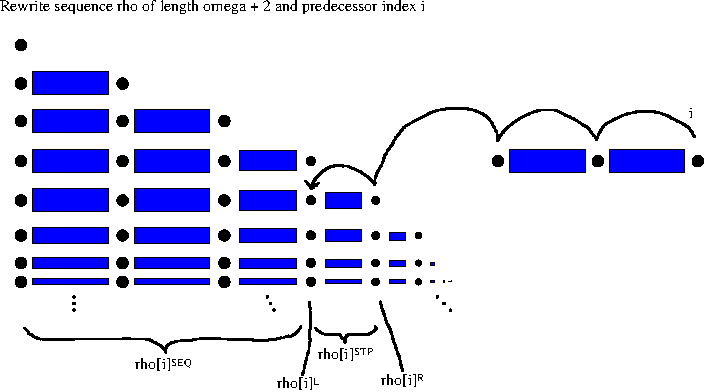
\includegraphics[draft=false]{predecessor.pdf}

% TODO: better wording for 'canceled out'?
Having a closer look at the order $\preceq$ on the Brouwer ordinals, we can
see that it really defines embeddings of their tree structures. This is due to
clause~\ref{def:order:succ} of Definition~\ref{def:order}. In this clause,
two occurrences of the $^+$ constructor (one in both ordinals) are canceled
out against each other, but the positions of these occurences in their
respective ordinals do not necessarily correspond. Since all occurrences of
$^+$ are equal, this has no effect on the resulting relation.

What this means for a translation of $\preceq$ to the domain of our
inductively defined rewrite sequences is that, indeed, we get an embedding
relation. We just have to make sure that in the
\coqref{Rewriting.Cons}{\coqdocconstructor{Cons}} case, we cancel out two
equivelent steps against each other.\footnote{A remark about equality on
  steps $\approx$.}
\begin{singlespace}
\begin{coqdoccode}
\coqdocnoindent
\coqdockw{Inductive} \coqdef{Rewriting.embed}{embed}{$\sqsubseteq$}
: \ensuremath{\forall} \coqdocvar{s} \coqdocvar{t} \coqdocvar{u}
\coqdocvar{v}, \coqdocvariable{s}
\coqref{Rewriting.sequence}{$\twoheadrightarrow_\mathcal{R}$} \coqdocvariable{t}
$\rightarrow$ \coqdocvariable{u}
\coqref{Rewriting.sequence}{$\twoheadrightarrow_\mathcal{R}$} \coqdocvariable{v}
$\rightarrow$ \coqdockw{Prop} :=\coqdoceol
\coqdocindent{1.00em}
\ensuremath{|}
\coqdef{Rewriting.EmbedNil}{Embed\_Nil}{\coqdocconstructor{$\sqsubseteq_\text{Nil}$}}  :
\ensuremath{\forall} \coqdocvar{s} \coqdocvar{u} \coqdocvar{v} (\coqdocvar{$\tau$}
: \coqdocvariable{u} \coqref{Rewriting.sequence}{$\twoheadrightarrow_\mathcal{R}$}
\coqdocvariable{v}),\coqdoceol
\coqdocindent{9.50em}
\coqref{Rewriting.Nil}{\coqdocconstructor{Nil}} \coqdocvariable{s}
\coqref{Rewriting.embed}{$\sqsubseteq$} \coqdocvariable{$\tau$}\coqdoceol
\coqdocindent{1.00em}
\ensuremath{|}
\coqdef{Rewriting.EmbedCons}{Embed\_Cons}{\coqdocconstructor{$\sqsubseteq_\text{Cons}$}} :
\ensuremath{\forall} \coqdocvar{s} \coqdocvar{t} \coqdocvar{u} \coqdocvar{v}
(\coqdocvar{$\tau$}
: \coqdocvariable{u} \coqref{Rewriting.sequence}{$\twoheadrightarrow_\mathcal{R}$}
\coqdocvariable{v}) (\coqdocvar{i} :
\coqref{Rewriting.predtype}{\coqdocdefinition{pred\_type}}
\coqdocvariable{$\tau$})
(\coqdocvar{$\rho$} : \coqdocvariable{s}
\coqref{Rewriting.sequence}{$\twoheadrightarrow_\mathcal{R}$}
\coqdocvariable{$\tau$}[\coqdocvariable{i}]$^\textsc{l}$)\coqdoceol
\coqdocindent{5.00em}
(\coqdocvar{$\pi$} :
\coqdocvariable{$\tau$}[\coqdocvariable{i}]$^\textsc{l}$
\coqref{Rewriting.step}{$\rightarrow_\mathcal{R}$}
\coqdocvariable{t}),\coqdoceol
\coqdocindent{9.50em}
\coqdocvariable{$\rho$} \coqref{Rewriting.embed}{$\sqsubseteq$}
\coqdocvariable{$\tau$}[\coqdocvariable{i}]$^\textsc{seq}$
\ensuremath{\rightarrow}\coqdoceol
\coqdocindent{9.50em}
\coqdocvariable{$\pi$} $\approx$
\coqdocvariable{$\tau$}[\coqdocvariable{i}]$^\textsc{stp}$
\ensuremath{\rightarrow}\coqdoceol
\coqdocindent{9.50em}
\coqref{Rewriting.Cons}{\coqdocconstructor{Cons}} \coqdocvariable{$\rho$}
\coqdocvariable{$\pi$} \coqref{Rewriting.embed}{$\sqsubseteq$}
\coqdocvariable{$\tau$}\coqdoceol
\coqdocindent{1.00em}
\ensuremath{|}
\coqdef{Rewriting.EmbedLim}{Embed\_Lim}{\coqdocconstructor{$\sqsubseteq_\text{Lim}$}}  :
\ensuremath{\forall} \coqdocvar{s} \coqdocvar{t} \coqdocvar{u} \coqdocvar{v}
(\coqdocvar{ts} :
\coqexternalref{http://coq.inria.fr/stdlib/Coq.Init.Datatypes}{nat}{\coqdocinductive{nat}}
\ensuremath{\rightarrow} \coqref{Term.term}{\coqdocinductive{term}})
(\coqdocvar{f} : \ensuremath{\forall} \coqdocvar{n},
\coqdocvariable{s}
\coqref{Rewriting.sequence}{$\twoheadrightarrow_\mathcal{R}$}
\coqdocvariable{ts} \coqdocvariable{n})\coqdoceol
\coqdocindent{5.00em}
(\coqdocvar{c} :
\coqref{Rewriting.converges}{\coqdocdefinition{converges}} \coqdocvariable{ts}
\coqdocvar{t}) (\coqdocvar{$\tau$} : \coqdocvar{u}
\coqref{Rewriting.sequence}{$\twoheadrightarrow_\mathcal{R}$}
\coqdocvar{v}),\coqdoceol
\coqdocindent{9.50em}
(\ensuremath{\forall} \coqdocvar{n}, (\coqdocvariable{f} \coqdocvariable{n})
\coqref{Rewriting.embed}{$\sqsubseteq$} \coqdocvariable{$\tau$}) \ensuremath{\rightarrow}\coqdoceol
\coqdocindent{9.50em}
\coqref{Rewriting.Lim}{\coqdocconstructor{Lim}} \coqdocvariable{f}
\coqdocvariable{c} \coqref{Rewriting.embed}{$\sqsubseteq$} \coqdocvariable{$\tau$}.\coqdoceol
\end{coqdoccode}
\end{singlespace}
% TODO: say what implicit/explicit arguments for cons and lim are


\subsection{Well-formed Sequences and Convergence}\label{sub:wf}

% TODO: this should not be in a subsection
On \coqref{Ordinal.ord}{\coqdocinductive{ord}} we defined the
\coqref{WfOrdinal.wf}{\coqdocdefinition{wf}} property to rule out a certain
class of ordinal representations. This issue translates directly to our
inductive representation of rewrite sequences.

$\sqsubseteq$ turns out to be satisfying for our present purposes.
